\documentclass[12pt]{article}
\usepackage{graphicx}
\usepackage {color}
\usepackage{pdfpages}
\usepackage{float}
\usepackage{changebar}
\usepackage{enumitem,amssymb}
\renewcommand{\familydefault}{\sfdefault}
\usepackage[margin=1.2in]{geometry}
\usepackage{graphicx}
\usepackage{wrapfig}
\usepackage[super]{cite}
\usepackage{subcaption}
\usepackage[table]{xcolor}
\usepackage{amsmath}
\usepackage[sort, numbers]{natbib}

%%%%%%%%%%%%Defining the margins %%%%%%%%%%%%%%%%%%%%%
\textheight 9.in
\textwidth 6.5in
\topmargin -.5in
\oddsidemargin 0in
\setlength{\parskip}{\smallskipamount}

%%%%%%%%%%%%%%Specific Commands %%%%%%%%%%%%%%%%%%
\newcommand{\eg}{{\em e.g.,}}
\newcommand{\ie}{{\em i.e.,}}
\newcommand{\etc}{{\em etc.,}}
\newcommand{\etal}{{\em et al.}}
\newcommand{\degrees}{{$^{\circ}$}}
\newcommand{\fig}[1]{\textbf{Figure #1}}

%%%%%%%%%%%%%%%%%%%%%%%%%%%% Setting to control figure placement
% These determine the rules used to place floating objects like figures 
% They are only guides, but read the manual to see the effect of each.
\renewcommand{\topfraction}{.9}
\renewcommand{\bottomfraction}{.9}
\renewcommand{\textfraction}{.1}
\renewcommand{\familydefault}{\sfdefault} %setting the san serif font

%%%%%%%%%%%%%%%%%%%%%%%% Line spacing
% Use the following command for ``double'' spacing
%\setlength{\baselineskip}{1.2\baselineskip}
% and this one for an acceptable NIH spacing of 6lpi based on 11pt
%\setlength{\baselineskip}{.9\baselineskip}
% The baselineskip does not appear to work when we include a maketitle
% command in the main file.  Something there must set the line spacing
% If we use this next command, then things seem to work.
\renewcommand{\baselinestretch}{.9}

\setcounter{secnumdepth}{0} %make no numbers but have a table of contents


\begin{document}

\title{Differences in Pharmaceutical vs Exercise Induced Ischemia: Implications for Development of Ischemic Models }

\author{Jake Bergquist, u6010393}
\maketitle

\section{Introduction}

%-Coronary Artery Disease affects (large number) annually
The detection and investigation of the electrophysiological consequences of myocardial ischemia has been a topic of active research for over a century as cardiac ischemia is a predictor of several potentially fatal heart conditions such as coronary artery disease, coronary artery dissection and others.\cite{BLZ:Saf2018,BLZ:Jes2013,BLZ:Noe2017,BLZ:Jes2012,RSM:Par20} Given the commonality of ischemia between many different heart conditions, its detection and diagnosis is a high impact area of medical research. Cardiac ischemia occurs when the supply of blood to a region of the heart is outpaced by the demand for nutrients such as oxygen. This can occur when a coronary artery become blocked partially or fully, or when some other change in flow occurs, or when the rate of metabolism increases past the ability of the coronary arteries to supply sufficient blood. The resulting lack of oxygen to the cardiac tissue leads the cardiomyocytes to become ischemic. If the ischemia does not persist its effects on the heart are reversible, thus it is critically important to diagnose and treat the ischemia quickly. The most predominant feature of ischemia that can be detected with non invasive methodology is changes in the ST segment of the ECG.\cite{RSM:Jan86a} When cardiomyocytes become ischemic there is a decrease in membrane voltage due to  mismanagement of ions within the cell. This results in a local elevation of the potential which is reflected primarily during the plateau phase of the myocardial action potential, which corresponds tot he ST segment of the ECG.\cite{RSM:Jan80} 

The common clinical methodology for the detection of myocardial ischemia is either an exercise or pharmaceutical stress test.\cite{Zenger2019,Beleslin1994} During such protocols stress is induced on the heart either by prolonged exercise or a chemical agent to increase heart rate. In the cases where the patient has some underlying ischemic condition this extra stress on the heart should induce changes on the body surface ECG that reflect the development of an ischemic are of myocardium. This will reflect in the ST segment of the ECG as cahnged in potential (typically elevations). While such tests are common they carry a strikingly accuracy (68-75\%) and a similarly low sensitivity (50--72\%) and specificity (69--90\%).\cite{BLZ:Knu2018a,RSM:Ste2002,BMB:Akk2011} Additionally it has been shown that ST and other ECG morphological changed based tests often show poor temporal performance.\cite{RSM:Goo2018} Thus while these exercise and pharmaceutical stress tests are the standard of care and commonly performed, there is striking evidence that they are not effective and that during such tests a heart that is ischemic remains ischemic for some time before ti can be detected. This can lead to potentially fatal complications. Clearly an increased understanding of the ischemia that develops during such stress tests is critical for improving the standard of care.

One potential area of interest for investigating the poor performance of these stress tests is the fact that while the two types of stress test (exercise or dobutamine infusion) are very different mechanisms of stress, they are treated as the same in the clinical setting. Indeed it has been shown that doubtamine and exercise stress tests induce different ischemia within the heart.\cite{Beleslin1994,Zenger2019} These studies suggest that a closer examination of these two ischemic conditions can improve our clinical understanding of the ischemia that is created, and thus we can better interpret the results of these clearly different stress tests.

A growing approach in modern electrocardiographic research at the whole organ and organism scale is computational modeling.\cite{RSM:Bur2018b} Such studies assist in understanding how different forms of ischemia can present in the context of ECG signals. Additionally these studies help to build a foundation for more advanced forms of electrocardiographic imaging (ECGI), whereby researchers and clinicians hope to be able to utilize non invasive imagining and measurement to localize cardiac electrical phenomena such as ischemia. By incorporating our understanding of the differences between the ischemia induced by these two different stress tests into a computational ischemic source model that predicts ecg signals we can better predict the response of an ischemic or ischmia prone heart to these different stressors. This will in turn improve our understanding of these different stress tests and improve their efficacy in the clinic.


\section{Background}

Myocardial ischemia is caused by inadequate blood flow to a region of myocardial tissue by the coronary arteries and capillaries. Whether it is caused by a blockage or disruption of blood flow, or an increase in metabolic demand by the heart that cannot be satisfied by the coronary arteries, the result is the same. The affected tissue becomes starved for oxygen and metabolic wast begins to accumulate. This results in a rise in trans-membrane potential. The rise in transmembrane potential results in a lower percentage sodium channels becoming de-inactivated at each action potential which in turns leads to a reduced amplitude action potential. This in combination with the increasing resting membrane potential results in a a potential difference between healthy and ischemic cells during the plateau phase. The currents that flow across this potential gradient give rise to elevations or depressions in the ST segment of the ECG as seen from either the myocardium or the body surface. \cite{RSM:Hea94,RSM:Jan80} Not only is this affected myocardial tissue not functioning at an optimum level, it is also highly arrhythmogenic which can easily lead to fatal cardiac arrhythmia or even sudden cardiac death.\cite{RSM:Jan80,Zipes98} The longer the ischemia persists the more the cells begin to shut down and eventually die.

In clinical practice a patient who is suspected of having a cardiac abnormality will be at the very least have their ECG read. However, the most common approach for diagnosing cardiac abnormalities, in particular any kind of ischemia, is a cardiac stress test. During these stress tests the patient is subjected to increasing cardiac demand until either they have reached the end of the testing protocol or substantial evidence of a problem is seen. The patient is hooked to a 12 lead ECG and asked to exercise on an inclined treadmill. The exercise causes a sympathetic increase in heart rate. Patients who are suffering from underlying ischemic condition or a condition that predisposes them to ischemia will likely develop an ischemic region within their myocardium. However it may be multiple minutes before this ischemia is detected on the torso surface, if it is detectable at all.\cite{RSM:Goo2018} Some patients are unable, physically or otherwise, to perform the exercise required by the stress test. In those cases the patient is administered a pharmaceutical agent that induces an increased heart stress, most commonly dobutamine, a $\beta$ receptor agonist. While these methods of stress are different they are clinically evaluated in the same way. Physicians examine the ECG to assess for ST segment changes alogn with any other beat morphology changes. However, research has shown that the ischemia produced is different, and the tests themselves respond differently in the clinic.\cite{Zenger2019,Beleslin1994} This difference in response for each other two stress tests raises several questions about botht he underlying physiology and the implications this has on the use of these stress tests clinically. Clearly, further investigation is necessary to determine how best to utilize these two clinical protocols in the assessment and diagnosis of myocardial ischemia.

Computational models provide a powerful tool for the exploration and understanding of various physiological systems. From modeling individual myocytes and other cardiac tissue, up to whole organ and individual scale models, simulation and computational modeling has many uses.\cite{TenTusscher2003,RSM:Bur2018b,Zenger2019} In the realm of ischemic modeling, researchers have worked to characterize the behavior of individual ischemic cells as well as how these cells behave on a whole heart level.\cite{BMB:Hop2004b,RSM:Bur2018b} By applying the principals derived from many cellular and organ scale research with physical mathematical models of the behavior of electric fields in biological medium researchers can model the potential distributions that would be detected by ECG and other recording electrodes under different ischemic conditions. This process, taking a known source of a signal (such as a know ischemic zone or a known heart surface potential) and projecting it onto another measurement surface is called the forward problem. The sources are used to solve a propagation of the electrical currents through the volume conductors of the heart and in some studies the torso using Laplace's equation in order to calculate what the potential distribution is on another surface.\cite{RSM:Bea2015a} These investigations lend insight into how different forms of ischemia can present clinically, and as a result this information can help shape diagnostic protocol. 

To date no research has explicitly applied the techniques of cardiac modeling to investigate the differences in exercise induced vs pharmaceutical induced ischemia. This exploration reviews two studies, Beleslin \etal\cite{Beleslin1994} in which researchers show that Dobutamine and exercise result in differences in the performance of stress testing and that the ischemia seen in each presents differently, and Burton \etal\cite{RSM:Bur2018b} in which researchers apply a passive monodomaine forward solution to solve3e for epicaridal potential distributions given a measured ischemic zone source within the myocardium. This review then suggests an integration of the methodologies and ideas presented in these two studies to achieve an improved understanding of stress test induced ischemia and how best to detect, diagnose, and interpret it.

%-Introduce how clinical stress tests are conducted and the difference between chemical and physical stress tests

%-Segment about ecgi in reference to stress tests

%-Introduce the concepts of computational modeling of ischemia on a whole heart scale


\section{Methods}
\subsection{Study 1: Clinical Study of Cardiac Stress Tests}
\paragraph{Subjects:}
In the study conducted  by Beleslin\etal\cite{Beleslin1994} 136 paitents were examined. Each of these paitents had been determined by coronary angiograph to have coronary artery obstruction, and by extension they were expected to show an ischemic response to a cardiac stress test. The subjects did not have any other history of heart failure, valvular heart disease, unstable angina, high blood pressure, or pulmonary dysfunction. Each patient was subjected to an exercise stress test as well as two pharmecutical based stress tests (dobutamine and dipyridamole) in a random order over the course of two days. The patients were monitored for their ECG, blood creatine kinase levels,  and presence of chest pain. A patient was diagnosed with acute ischemia if two of the three diagnosis criteria presented: definitive signature of ischemia on the ECG (changes in the ST segment), a characteristic pattern of rise and fall of blood serum creatine kinase levels, and/or persistent angina or chest pain lasting more than thirty minutes.

\paragraph{Stress Tests:}
The exercise stress test was performed according to the Bruce treadmill protocol. The patient was asked to run on a treadmill with the incline and speed to increase in a step-wise fashion. This would induce a step-wise increase in the demand placed on the heart. The protocol was continued until either ischemia was detected, exhaustion, another cardiac phenomena was observed, or another circumstance that required cessation arose. For the pharmaceutical stress test the patients were infused intravenously with either doubtamine or dipyridamole with an increase in rate every 3 minutes. The infusions were terminated at the onset of any severe symptoms or the detection of ischemia. 

\paragraph{Monitoring and Analysis}
Patients were monitored via ECG and echocardiogram, blood pressure, heart rate, and a qualitative description of symptoms. Double product was calculated as the product of systolic blood pressure and heart rate. All statistic were calculate using ANOVA , 2 sample T test, and Newman-Keuls test.


\subsection{Study 2: }
\paragraph{Ischemic Animal Model:}
In the study conducted by Bruton \etal utilized a canine ischemia experimental preparation. An anesthetized canine subject's heart was exposed by a sternotomy. The left anterior descending LAD) coronary artery was dissected and a calibrated hydrolic occluder was wrapped around the LAD. A flexible epicardial sock electrode array was fit over the heart. This sock had stitched into it 247 unipolar recording electrodes spaced roughly 3 mm apart. Transmural plunge needles were place into the myocardium into the assumed perfusion bed of the LAD. These needles have 10 evenly spaced unipolar electrodes along the shaft that record from the 3D extend of the myocardium. Ischemic stress is induced by occlusion of the hydrolic occluder and pacing from the right atria. In total 226 episodes of ischemia were induced and analyzed across several canine subjects.

\paragraph{Data Processing:}
Post experiment a subset of sock electrodes were digitized using a mechanical digitizer (which records the 3D location of the electrodes) and the heart was excised. High resolution imaging was acquired of the heart using FISP, FLASH, and DTI imaging protocols. The FISP and FLASH protocols produce images that can be segmented and meshed to produce a 3D heart mesh for computation. The DTI (diffusion tensor imaging) scans are used to calculate the principle fiber direction for incorporation into the mathematical computations. The signals collected from the needle electrode arrays were utilized to identify an ischemic zone. The ST40\% time point (40\% into the ST segment) was used to identify electrodes that were ischemic. These nodes were meshed into an ischemic volume. The sock recording array was used to validate the calculated epicardial potential distribtuoins from the resulting forward model calculation.

\paragraph{Forward Model:}
This study employed a passive monodomain formulation for calculating the epicardial potentials from the ischemic source. This formulation leverages Equation~\ref{EQ1} in which $\sigma_e$ represents the extracellular conductivity and $\phi_e$ represents the extracellular potentials. A subset of the extracellular potentials were the known ST40\% values of the ischemic zone which were then used to calculate the remaining extracellular potentials throughout the cardiac volume. Boundary conditions were set at the heart surface (no current flow outside of the heart) the blood/myocardium interface (current allowed to flow into the blood). By solving Eq~\ref{EQ1} for all other extracellular potentials the epicardiul potential distribution could be calculated.
\begin{equation}
\nabla\cdot(\sigma_e\nabla\phi_e) = 0
\label{EQ1}
\end{equation}

\paragraph{Analysis:}
The calculated epicardial potential distribution was compared to the measured epicardial distribution at the ST40\% time. These distributions were compared based on Pearson's correlation coefficient (PCC), root-mean-square error (RMSe), and maximum absolute error ($AE_{max}$). Additionally the measured and calculated potential distributions on the epicardium were visualized in order to make qualitative assessments of the results.

\section{Results}
\subsection{Study 1}
Figure~\ref{p1r1} summarizes the measurements of study 1 where we can see that for each of the three stress tests the physiological parameters measured varied. The asterisk denotes parameters that varied significantly (P < 0.01) across the three stress protocols. Figure~\ref{p1r2} shows the sensitivity, specificity, and accuracy of each of the three protocols tested. As can be seen the sensitivity and accuracy is significantly different between exercise and dipyridamole stress. Additionally while not reported as significant there is some variability in the performance of dobutamine with respect to exercise based stress.
\begin{figure}[H]
	\centering
	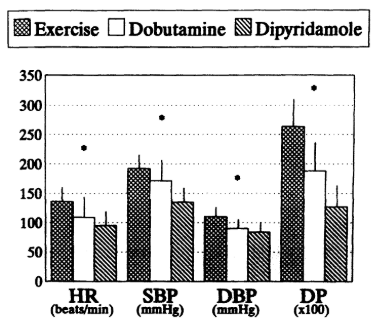
\includegraphics[width = (0.8\textwidth)]{Figures/Paper1Result1.png}
	\caption{Bar Chart showing differences in heart rate, systolic blood pressure (SBP), diastolic blood pressure (DPB), and double product (DP) for each of the three stress tests. Figure from \cite{Beleslin1994}}
	\label{p1r1}
\end{figure}

\begin{figure}[H]
	\centering
	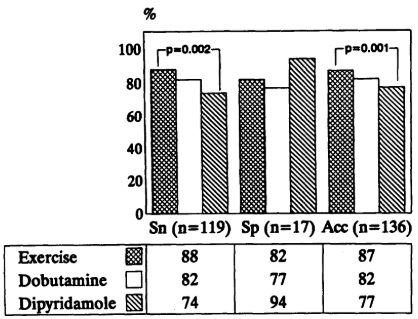
\includegraphics[width=(0.8\textwidth)]{Figures/Paper1Result2.png}
	\caption{Bar chart and table of sensitivity (sn), specificity (sp), and accuracy (acc) of the three stress tests in regards to detecting myocardial ischemia. Figure from \cite{Beleslin1994})}
	\label{p1r2}
\end{figure}

The investigations in Beleslin \etal report that despite the differences observed pharmaceutical stress tests could be substituted for the exercised based test without major issue. Via their ecocardiographic study they also assess that the area of the heart that was affected by the ischemia was similar between each stress protocol, as measured by the area of the heart that became less active during the stress protocol.

\subsection{Study 2}
The visualization results presented in Figure~\ref{p2r1} show agreement between the simulated and measured epicardal potentials during an ischemic intervention, particularly in the region sampled by the needle electrode arrays. However,  the simulated potentials are not perfect and some complex morphologies of the potential distribtuin are not captured by the simulation, particularly the posterior depression as seen on the measured signals. The numerical results are summarized in Figure~\ref{p2r2} which shows a range of PCC values. Generally the simulated potential distributions whose maximum voltage was less that 3.5 mV resulted in superion PCC values as seen in Figure~\ref{p2r3}.

\begin{figure}[H]
	\centering
	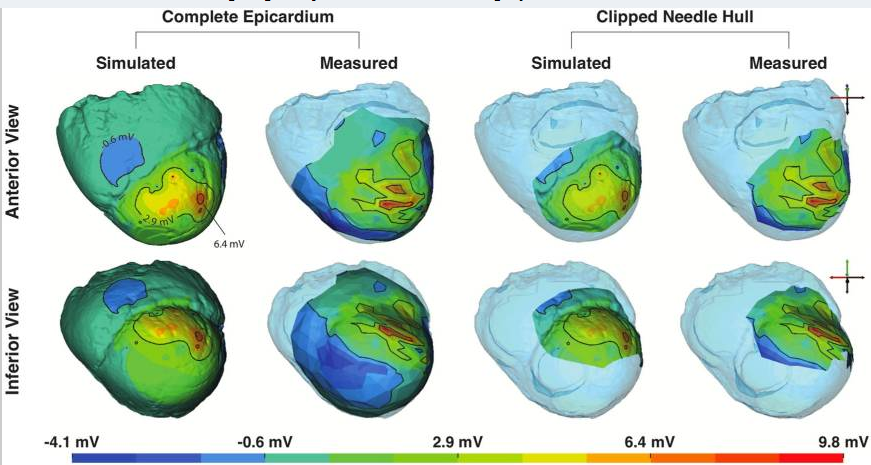
\includegraphics[width=(\textwidth)]{Figures/Paper2Result1.png}
	\caption{Epicardial potentials from measured and simulated ST40\% time points. The first two columns show visualizations of the entire epicardium. The second two columns show the potentials only mapped into the area covered by the transmural plunge needle electrodes. Figure from \cite{RSM:Bur2018b}}
	\label{p2r1}
\end{figure}

\begin{figure}[H]
	\centering
	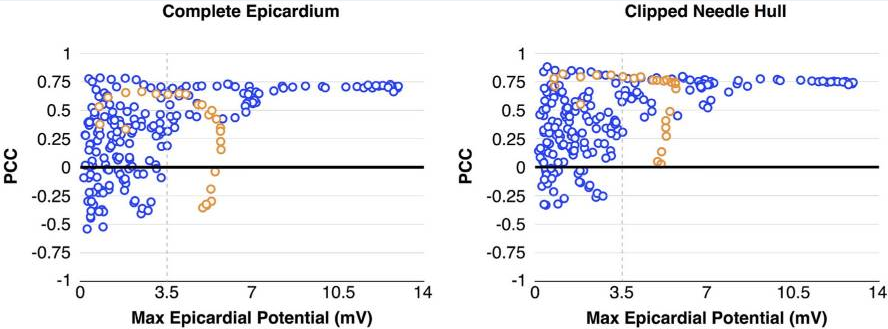
\includegraphics[width=(\textwidth)]{Figures/Paper2Result2.png}
	\caption{Pearson's correlation coefficient vs maximum epicardial potential for both the full epicardium and the needle hull zone, the are covered by the transmural needle electrodes. Blue markers show the typical ischemic interventions. The orange markers show a series of sequential ischemic interventions that involved an atypical trend where increased ischemic stress resulted in increased peak potential but a dramatically decreasing PCC. Figure from \cite{RSM:Bur2018b}}
	\label{p2r2}
\end{figure}
\begin{figure}[H]
	\centering
	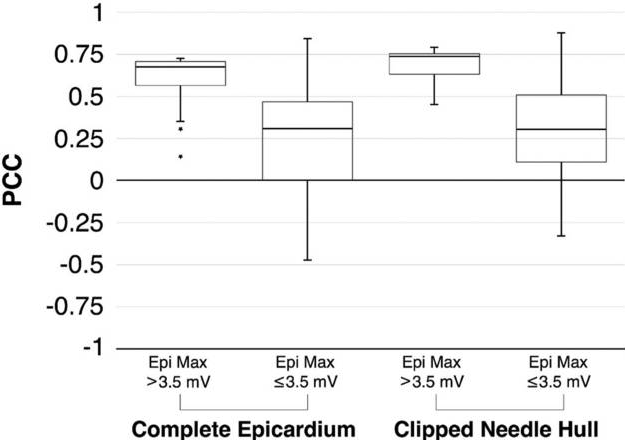
\includegraphics[width=(\textwidth)]{Figures/Paper2Result3.png}
	\caption{Pearson's correlation coefficient at different maximum epicardial potential thresholds. Figure from \cite{RSM:Bur2018b}}
	\label{p2r3}
\end{figure}


%-paper concludes that despite these differences chemical stressors can serve in place of exercise stress tests in patients who are unwilling/unable to perform the standard Bruce exercise stress test.

%Paper 2:

%-was able to recapitulate ischemic extracellular potentials on the epicardium using modeled ischemic transmembrane sources. Demonstrated that the passive bidomain can be used to model ischemia within the heart.


\section{Discussion}

%-While paper 1 concludes that the stress tests examined are all adequate for detecting ischemia, there are clear differences in the pysiological response. This implies a difference in the ischemia induced. This idea of different ischemia produced by different stress tests is supported by other studies.\cite{Zenger2019}
Study 1 set out to assess the efficacy and evaluate the differences between three different ischemic stress protocols used clinically. As can be seen in Figure~\ref{p1r1} there are significant differences in heart rate, blood pressure, and double product (which just another measure of heart rate and blood pressure). Clearly the effects these stressors are having on the body are different, and as a result one might infer that the underlying ischemia induced is different despite it being within the same patient. This idea of chemical vs exercise based stressors causing different ischemia to form is supported by other preliminary work.\cite{Zenger2019} The investigators of study 1 concluded that while the pharmaceutical methods were less robust they produced comparable results to the exercise based testing. The researchers also asserted that utilizing the echocardiograph provided superior investigation of the ischemic response, but given the feasibility and availability of ECG as a diagnostic tool it makes sense to focus on the ECG as a point of development for future diagnostic tools. This study is limited in several ways. The study did not include a control of testing patients who showed no signs of ischemia to provide a background and a way of assessing false positive rate for each protocol. Additionally the resolution available with echocardiography and the limited analysis performed makes these results less convincing. Without any direct analysis of the electrical potential distribution on and within the heart it is difficult to make full conclusions about the physiologic differences between these stress tests. This limitation stems from the fact that this study utilized human subjects, for which only non-invasive procedures could be considered. A main takeaway from this study is that the physiologic response to these different ischemic stress tests is different. Additionally there is variability in the accuracy of each of these tests. A potential mechanism to explain the difference in these stress tests is the fact that during a standard exercise stress test the skeletal muscles are experiencing metabolic demand in addition to the heart. This cascade of signaling is likely different than what occurs during a pharmaceutical test in which the subject is exerting no physical effort. Additionally stressors like dobutamine can have off target effects and create scenarios not indicative of typical physiology.

This study leaves many open questions. It is curious that there are significant differences in the physiological parameters (blood pressure, heart rate) measured. What are the other physiological differences, and particularly what are the electrical differences? Do the body surface potential maps look vastly different or similar during these episodes of ischemia? How can we use this information to better assess clinically induced ischemia? If researchers apply more rigorous methods to differentiate and parameterize the ischemia induced by these different stress methods it is likely that some general improvements to the diagnosis protocols could be made. At the very least the electrocardiographic differences between these ischemia types should be addressed by a technique such as that seen in study 2. 


Study 2 set out to utilize experiment specific ischemic zones recorded during experimentally induced cardiac ischemia to simulate the epicardial potentials. These simulated potentials were then compared to measured potentials. The study demonstrates appreciable agreement between simulated and measured values and potential distributions. By parameterizing an ischemic zone the researchers were able to recreate ischemic potentials on the heart surface. This study is limited in its clinical translateability as the potentials were not fully forward computed to the torso surface. Additionally the ischemic interventions utilized were not modeled after any clinical ischemic stress tests, which would be desirable in translating these results into clinical significance. What this study does is establishes a framework for computing potential distributions from an ischemic zone. This framework could easily be extended to calculate the potentials on a simulated torso geometry in order to assess how these ischemic sources reflect int he torso suface potential distributions and ECG signals. 

Study two raises some questions. When we consider Figure~\ref{p2r1} we see that the simulation method was unable to prduce the measured depression on the apical posterior region of th epicardium. What could be the cause for this discrepancy? There is a possibility that the ischemic zone chosen or the formulation of the mono domain is insufficient to recreate this signal morphology. It is also possible that the needle electrodes used did not sample the entire ischemic source, and as such there are complexities of the potential distribution that cannot be recaptured as the simulation is missing data. a potential improvement would be to utilize a more complex bidomain model that formulates the simulation in terms of extracellular and intracellular potentials. Additionally utilizing a larger number of needles to get a wider and more dense coverage to achieve higher spatial resolution and coverage. Another question would be what does the ischemia created by the standard ischemic stress protocols such as those discussed in Study 1, look like at the resolution examined by study 2. This question leads to an integration of the ideas of both studies that would allow for an interesting investigation of the key topics covered by both studies.

A powerful integration of the ideas present in these studies would be to perform ischemic stress experiments in a large animal preparation with different clinically based stress tests then utilize the simulation pipeline from Burton \etal to model the ischemia created. The study of Burton \etal could then be extended to project the calculated epicardial potentials onto a torso surface to allow for the assessment of what these different ischemic stress protocols look like on a torso surface ECG. This extension would be easy to perform utilizing a similar forward simulation through a torso geometry or even a different method such as boundary element calculation. The result of this integration would be a study that utilizes computational modeling to investigate the effects of different clinically derived ischemic stress protocols on body surface potentials. By parameterizing the ischemic source by the different stress test protocols one could hope to elucidate the differences between the different stress tests based on the ischemic zones identified. By applying the framework developed by Burton \etal the electrophysiological differences between the induced ischemia could be more closely investigated. These results would likely better inform the interpretation of the ECGs taken during these stress tests and result in improved diagnosis of myocardial ischemia.

Both studies independently have demonstrated significant development of our knowledge of myocardial ischemia, how it forms, and what it looks like. Future studies in this area are still needed to fully elucidate the nature and complexities of myocardial ischemia both in stress test scenarios and others. These papers highlight two aspects of ischemia research, study 1 being more clinically minded and study 2 being computationally and physiologically driven. It is only by the integration of both realms can we come to a full understanding of myocardial ischemia and thereby formulate the most effective diagnostic and treatment tools.


%-Paper 1 highlights the need to further investigate these differences. By applying the method of paper 2 we may gain a deeper understanding of the ischemia that developed. As a consequence of this proposed integration the findings may inform clinicians on how better to interpret the results of the different stress tests, leading to more accurate and effective diagnosis of cardiac ischemia.

%%%%%%%%%%%%%%%%%% Correct Bibliography Style
\bibliography{library,biglit,blz,bmb}
\bibliographystyle{IEEEtran}


\end{document}








